%# -*- coding:utf-8 -*-
\chapter{面向虚拟交互的血管模型优化}
\label{chap6}

\section{Introduction}

%Coronary heart diseases () are among the most fatal illnesses worldwide \cite{WHO2013}.
%The diseases occur when the stenosis or even blockages formed due to the build up of fatty substances on the inner wall of the blood vessels.
Percutaneous coronary intervention (PCI) is the gold standard in fighting the coronary heart diseases, which is one of the most lethal diseases in the modern world \cite{WHO2013}. %
Due to the minimally-invasive traits, this procedure causes smaller incision and much less trauma to the patients than open surgery performed in the past.
%In addition, the hospitalization after the procedure is in turn dramatically shortened.
However, this feature also makes it hard for the learners to get used to it.
Besides, after entering the real catheterization labs, the clinicians have to endure the potential occupational hazards year after year \cite{Smilowitz2012}.
%They typically need strict and long term training before performing the procedure on real patient. %
%What's worse, the practitioners in catheterization labs have to expose themselves under the ionizing radiation from the fluoroscope while examining the morphologies of the patients' vasculature. %

In this context, robot-assisted intravascular system came into play with the aim of changing this situation.
With these robots \cite{Beyar2006RNS,Smilowitz2012}, the work load of the cardiologists are dramatically lightened, and the risks of their health are greatly decreased.
However, as their ancient manually performed counterparts, the technique of steering the robotic arms in surgery is still hard for the novice.

Traditional paradigm of PCI training strictly followed the physical fashion -- performing demonstrative procedure on biological or non-biological models \cite{Lunderquist1995,Mori1998}. %
The former materials, including unclaimed cadavers and live animals, are ethic-disputed.
Moreover, the expenditure on the preservation and feeding is high-rising, and the distinction in anatomy between human and animal volunteer is apparent even for the amateur. %
The latter are rigid and stiff both in touching and looking.

In the case of training of robotic systems, one fact is that the advanced robotic systems can not be applied to the training for the health of the clinicians and the lives of the patients will be at risk. %
In order to solve this problem, better training vehicles are required.
Thanks to the advancement of computer hardware, we could employ the greatly improved computer system as the platform, on which the dedicated computer-aided training simulation can be realized. %

Our aim is to implement a computer-aided simulation training system for the minimally-invasive intravascular robotic system built in our lab \cite{Ji2011EMBC}.
In realizing this training platform, the temporal performance of interaction between the anatomic structures in computing environment (e.g., the vascular system) and the virtual surgical tools are undoubtedly of the primary concern. %
In order to improve this performance, the quantity of the consisting polygons needed to be greatly reduced.

In this paper, we developed an approach to substantially eliminate the total number of the polygonal elements of the vasculature model.
As the most popular primitive for the modern computer graphics application, the polygons can be rendered in any standard commercial computer graphics systems.
The fact is that in surface rendering, the more precise the results are, the more polygons are required.
This makes the rendering of the huge amount of polygons occupy too much computation resources, especially the memories.
In the field of medical visualization and simulation, models rendered using surface techniques require even more polygons to capture various of complex and delicate human anatomic structures. %
The decimation algorithm introduced in our work is an application independent method to eliminate the polygons (especially triangles) by performing local operations \cite{Schroeder1992}. %

The input data is the patient-specific surface model of the human vasculature based on the computed tomography angiography (CTA).
Firstly, the connectivity of the polygons that consisting the surface is validated thoroughly to include the largest connected polygons that is effective in representing the surface. %
Secondly, the uneven surfaces are smoothed in order to reduce the unnecessary effects on the following decimation.
Finally, numbers of the component polygons of the vessel model are eliminated.
The capability of our approach in reducing the amount of polygonal components of the vessel model is proved by the experimental results.

The remainder of this paper is organized as follows.
Section II outlines the work flow and describes the techniques introduced in this work.
Section III describes the experiments and presents the results, ending with a discussion.
The final section concludes the whole work and outlooks the future plans.

\section{Methodologies}

\subsection{Overview}

This section discusses the layout of the main methods used in processing and optimization of the meshes consisting the model surface.
The surface model of the vasculature used in this work was generated from the CTA information which was acquired from some real patient.
In order to put the model into the use of virtual interaction, the amount of information of the model have to be limited because of the constraints of the graphics hardware.
To limit the amount of information is equivalent to eliminate the total number of the polygonal elements that consist the model as much as possible, while preserving the original geometry of the vasculature. %

Some preprocessing steps illustrated in Fig. \ref{fig:DataFlow} are necessary before the elimination of the polygons in the surface.
First of all, the validation of the connectivity among the vertices in the image-based model surface are performed to guarantee that the surface to be processed is complete as a whole and all the vertices are connected. %
Secondly, the smoothing step is introduced in order to depress the bulges and sunken areas in the connected surface.
Finally, the polygonal elements in the surface model are selected and part of them are deleted; the ``holes" left are patched and the geometry of the model is preserved as complete as possible. %

\subsection{Connectivity Validation}

Before any processing steps, one routine must be done to ensure that the surface model considered is well-shaped that no extra polygons exist in defining the same piece of surface.
This routine is designed to extract the polygons based on the geometric connectivity.
Concretely, it can extract the cells (i.e., polygons and/or triangles) that share the common points (i.e., vertices).

\subsection{Surface Smoothing}

In the field of computer graphics and imaging, the visualization of curves and surfaces (both will be referred to as \emph{shapes}) both in two- or three-dimensional space are common, especially for the volumetric data from medical field. %
The computation is in fact the proper approximation of the original shapes by the polygonal curves or polyhedral surfaces.
Typically, artifacts at certain level can be found in the resultant approximating shapes (see Fig. \ref{fig:Artifact}), and can be smoothed while maintaining the overall geometry (see Fig. \ref{fig:ArtifactRemoved}). %
In this work, one of our objectives is the smoothing or fairing of the model surface acquired by applying the iso-intensity extraction techniques on the raw medical images.
\begin{figure}[t]
\centering
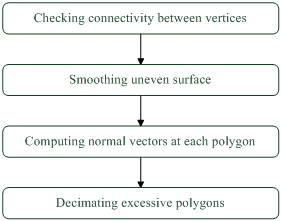
\includegraphics[width=3.2in]{Figures/chap06/DataFlow.png}
\caption{Overview of the work flow.}
\label{fig:DataFlow}
\end{figure}
\begin{figure}[t]
\centering
\subfloat{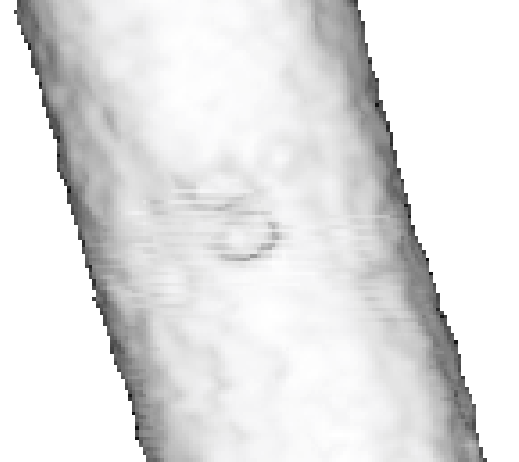
\includegraphics[height=1.0in]{Figures/chap06/artifact.png}%
\label{fig:Artifact}}
\hfil
\subfloat{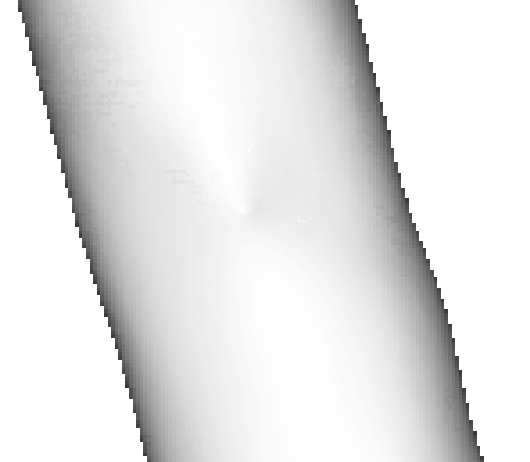
\includegraphics[height=1.0in]{Figures/chap06/artifact_removed.png}%
\label{fig:ArtifactRemoved}}
\caption{Smoothing the artifacts due to the approximation in visualization. (a) the artifacts (the horizontal ``steps" on the model surface of the vasculature); (b) the results after the smoothing process.}%
\label{fig:ArtifactComparison}
\end{figure}
A signal processing approach is employed to fulfill this task.
The approach is actually a linear low-pass filtering technique \cite{Taubin1995ICCV}, which is a low-level processing in the field of digital signal processing.
It can be applied to the smoothing process on the curves/surfaces of arbitrary dimension and complexities in geometry.
Moreover, no shrinkages will be introduced by the method during the computation.

The method is built upon the concepts of \emph{discrete graph signal} and its three-dimensional counterpart, \emph{discrete surface signal} \cite{Taubin1995SIG}.

By discrete graph signal, it means that some functions defined on the directed graph (\emph{digraph} for short).
Corresponding the polyhedral surfaces in consideration, the digraph $G$ can be marked as $G: \left\{ V_g, E\right\}$, where $V_g = \left\{ 1, \ldots, n \right\}$ is \emph{vertex set} including all the vertices in the graph, labeled from $1$ to $n$; and $E$ is the \emph{edge set} including the edges between any pair of vertices in the set $V_g$. %
The so-called discrete graph signal is a $n$-dimensional vector $x = \left[ x_1, \ldots, x_n \right]^T$, where the component $x_i, i = 1, \ldots, n$ denotes the signal intensity at the vertex $i \in V_g$. %

By discrete surface signal, it means that some functions defined on the polyhedral surfaces.
The polyhedral surfaces $S$ can be represented as $S: \left\{ V_s, F\right\}$, where $V_s = \left\{ 1, \ldots, n \right\}$ is \emph{vertex set} including all the vertices in the polyhedral surfaces, marked from $1$ to $n$; and $F$ is the set including the faces surrounded by the vertices in the set $V_s$ and the edges connecting them. %
The discrete surface signal is a $n$-dimensional vector $y = \left[ y_1, \ldots, y_n \right]^T$, where the component $y_j, j = 1, \ldots, n$ corresponds to the signal value at the vertex $j \in V_s$. %

For the smoothing of the planar polygonal curves, the classical Fourier analysis can be applied to decompose the original curves into orthogonal subspaces with distinct frequencies. %
After that, the components at high frequencies are removed as noises and the ones at low frequencies are left.
The idea can be extended to the case of the polyhedral surfaces with arbitrary topology.

For the discrete surface signal $y$, the weighted Laplacian operators for the vertices in $V_s$ are defined as
\begin{equation}
\label{eqn:Laplacian}
\Delta y_i = \sum_{j \in i^{\ast}} w_{ij} \left( y_j - y_i \right),
\end{equation}
where $w_{ij}$ is the positive weight for $y_j - y_i$, and for any $i$, the sum of its weights are always one, $\sum_{j \in i^{\ast}} w_{ij} = 1$.
The matrix form of (\ref{eqn:Laplacian}) is
\begin{equation}
\label{eqn:LaplacianMatrix}
\Delta y = - K y,
\end{equation}
where $K = I - W$, with $W$ the matrix of weights and $I$ an identity matrix.
Here we define $0 \leq \lambda_1 \leq \ldots \leq \lambda_n \leq 2$ as the real eigenvalues of $K$, and $e_1, \ldots, e_n$ the corresponding unit right eigenvectors.

At this point, the low-pass filtering can be presented as the multiplication of the matrix function $f(K)$ by the input signal $y$:
\begin{equation}
\label{eqn:LowPassEquivalent}
y' = f(K) y.
\end{equation}
For any polynomial transfer function, the output signal in (\ref{eqn:LowPassEquivalent}) can be rewritten as
\begin{equation}
\label{eqn:LowPassPolynomial}
y' = \sum_{i=1}^{n} \rho_i f(k_i) e_i,
\end{equation}
where $\rho_i$ are the coefficients of the linear combination of the unit right eigenvectors of the input signal $y$: $y = \sum_{i} \rho_i e_i$.
In order to realize a low pass filter, $f(k_i)$ is designed to satisfy two conditions: for $k_i \in [0,2]$, $f(k_i) \approx 1$ for low frequencies; $f(k_i) \approx 0$ for high frequencies. %

The low-pass filtering mechanism can be achieved by adjusting the weights in the following polynomial approximation \cite{Taubin1996}:
\begin{equation}
\label{eqn:Approximation}
f_{N}(k) = w_0 \frac{\theta}{\pi} T_0 (1 - k / 2) + w_n \sum_{n} \frac{2 \sin (n \theta)}{n \pi} T_n(1 - k / 2),
\end{equation}
where $\theta$ is the unique solution of $k = 2 (1 - \cos \theta)$ on $[0, \pi / 2]$, and $T_0(\cdot)$ and $T_n(\cdot)$ are the Chebyshev polynomials.
Here in this work, the weights in (\ref{eqn:Approximation}) is adjusted to form a Hamming window \cite{Taubin1996}, which can be represented as follows:
\begin{equation}
\label{eqn:HammingWindow}
w_n = 0.54 + 0.46 \cos (n \pi / (N + 1) ).
\end{equation}

After smoothing the surface, the normal vectors (\emph{normals} in short) are computed for each polygonal mesh.

\subsection{Polygons Decimation}
\label{subsec:decimation}

To eliminate the total number of polygons that consisting the model surface, an algorithm for the decimation of triangle meshes is employed in our approach \cite{Schroeder1992}.
The algorithm attempts to decimate certain rate of original meshes by firstly deleting the vertices whose coordinates are validated beforehand in the surface and then patching the holes left by creating a new triangulation at the location. %

All the vertices are labeled as simple, complex, and corners (see Fig. \ref{fig:FiveClasses}).
For simple vertices, two special cases are further specified as boundary vertices, and interior edge vertices.
\begin{figure}[t]
\centering
\subfloat{
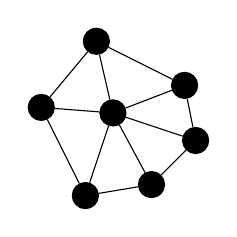
\begin{tikzpicture}[scale=.7,every node/.style={draw,shape=circle,fill=black,minimum size=1pt}]
% vertices
\path (0.5,1.5) node (p0) {}
(0,0) node (p1) {}
(1.2,0.2) node (p2) {}
(2,1) node (p3) {}
(1.8,2) node (p4) {}
(0.2,2.8) node (p5) {}
(-0.8,1.6) node (p6) {};
% edges
\draw (p0) -- (p1)
(p0) -- (p2)
(p0) -- (p3)
(p0) -- (p4)
(p0) -- (p5)
(p0) -- (p6)
(p1) -- (p2)
(p2) -- (p3)
(p3) -- (p4)
(p4) -- (p5)
(p5) -- (p6)
(p6) -- (p1);
\end{tikzpicture}
\label{fig:GeneralSimple}
}
\hfil
\subfloat{
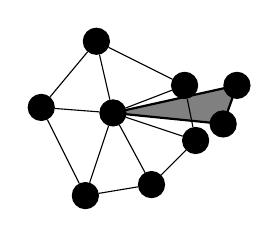
\begin{tikzpicture}[scale=.7,every node/.style={draw,shape=circle,fill=black,minimum size=1pt}]
\draw [fill=gray,thick] (0.5,1.5) -- (2.5,1.3) -- (2.75,2) -- (0.5,1.5);
% vertices
\path (0.5,1.5) node (p0) {}
(0,0) node (p1) {}
(1.2,0.2) node (p2) {}
(2,1) node (p3) {}
(1.8,2) node (p4) {}
(0.2,2.8) node (p5) {}
(-0.8,1.6) node (p6) {}
(2.5,1.3) node (p7) {}
(2.75,2) node (p8) {};
% edges
\draw (p0) -- (p1)
(p0) -- (p2)
(p0) -- (p3)
(p0) -- (p4)
(p0) -- (p5)
(p0) -- (p6)
(p1) -- (p2)
(p2) -- (p3)
(p3) -- (p4)
(p4) -- (p5)
(p5) -- (p6)
(p6) -- (p1);
\end{tikzpicture}
\label{fig:Complex}
}
\hfil
\subfloat{
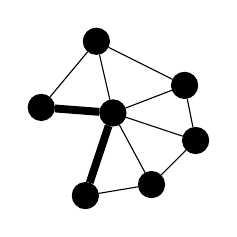
\begin{tikzpicture}[scale=.7,every node/.style={draw,shape=circle,fill=black,minimum size=1pt}]
% vertices
\path (0.5,1.5) node (p0) {}
(0,0) node (p1) {}
(1.2,0.2) node (p2) {}
(2,1) node (p3) {}
(1.8,2) node (p4) {}
(0.2,2.8) node (p5) {}
(-0.8,1.6) node (p6) {};
% edges
\draw (p0) -- (p1)
(p0) -- (p2)
(p0) -- (p3)
(p0) -- (p4)
(p0) -- (p5)
(p0) -- (p6)
(p1) -- (p2)
(p2) -- (p3)
(p3) -- (p4)
(p4) -- (p5)
(p5) -- (p6);
\draw [line width=.1cm] (p1) -- (p0) -- (p6);
\end{tikzpicture}
\label{fig:Boundary}
}
\hfil
\subfloat{
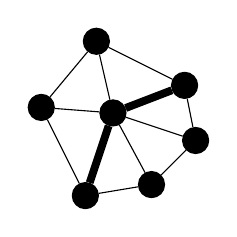
\begin{tikzpicture}[scale=.7,every node/.style={draw,shape=circle,fill=black,minimum size=1pt}]
% vertices
\path (0.5,1.5) node (p0) {}
(0,0) node (p1) {}
(1.2,0.2) node (p2) {}
(2,1) node (p3) {}
(1.8,2) node (p4) {}
(0.2,2.8) node (p5) {}
(-0.8,1.6) node (p6) {};
% edges
\draw (p0) -- (p1)
(p0) -- (p2)
(p0) -- (p3)
(p0) -- (p4)
(p0) -- (p5)
(p0) -- (p6)
(p1) -- (p2)
(p2) -- (p3)
(p3) -- (p4)
(p4) -- (p5)
(p5) -- (p6)
(p6) -- (p1);
\draw [line width=.1cm] (p1) -- (p0) -- (p4);
\end{tikzpicture}
\label{fig:InteriorEdge}
}
\hfil
\subfloat{
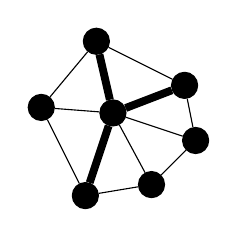
\begin{tikzpicture}[scale=.7,every node/.style={draw,shape=circle,fill=black,minimum size=1pt}]
% vertices
\path (0.5,1.5) node (p0) {}
(0,0) node (p1) {}
(1.2,0.2) node (p2) {}
(2,1) node (p3) {}
(1.8,2) node (p4) {}
(0.2,2.8) node (p5) {}
(-0.8,1.6) node (p6) {};
% edges
\draw (p0) -- (p1)
(p0) -- (p2)
(p0) -- (p3)
(p0) -- (p4)
(p0) -- (p5)
(p0) -- (p6)
(p1) -- (p2)
(p2) -- (p3)
(p3) -- (p4)
(p4) -- (p5)
(p5) -- (p6)
(p6) -- (p1);
\draw [line width=.1cm] (p1) -- (p0) -- (p4);
\draw [line width=.1cm] (p0) -- (p5);
\end{tikzpicture}
\label{fig:Corner}
}
\caption{Five classes of the vertex in the surface. (a) General simple case; (b) Complex case; (c) Boundary case; (d) Interior edge case; (e) Corner case. }%
\label{fig:FiveClasses}
\end{figure}
\begin{figure}[t]
\centering
\subfloat{
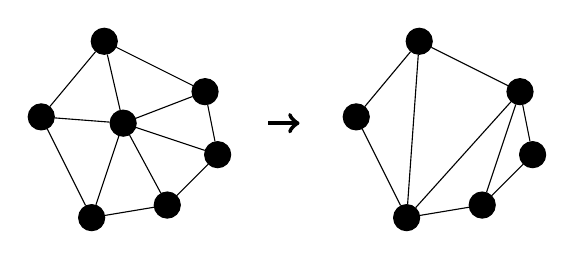
\begin{tikzpicture}[scale=.8,every node/.style={draw,shape=circle,fill=black,minimum size=3pt}]
% vertices
\path (0.5,1.5) node (p0) {}
(0,0) node (p1) {}
(1.2,0.2) node (p2) {}
(2,1) node (p3) {}
(1.8,2) node (p4) {}
(0.2,2.8) node (p5) {}
(-0.8,1.6) node (p6) {};
\path %(5.5,1.5) node (p7) {}
(5,0) node (p8) {}
(6.2,0.2) node (p9) {}
(7,1) node (p10) {}
(6.8,2) node (p11) {}
(5.2,2.8) node (p12) {}
(4.2,1.6) node (p13) {};
% edges
\draw (p0) -- (p1)
(p0) -- (p2)
(p0) -- (p3)
(p0) -- (p4)
(p0) -- (p5)
(p0) -- (p6)
(p1) -- (p2)
(p2) -- (p3)
(p3) -- (p4)
(p4) -- (p5)
(p5) -- (p6)
(p6) -- (p1);
\draw (p8) -- (p9)
(p9) -- (p10)
(p10) -- (p11)
(p11) -- (p12)
(p12) -- (p13)
(p13) -- (p8)
(p8) -- (p12)
(p8) -- (p11)
(p9) -- (p11);
% draw arrow
\draw [->,ultra thick] (2.8,1.5) -- (3.3,1.5);
\end{tikzpicture}
\label{fig:SimpleReduction}
}
\hfil
\subfloat{
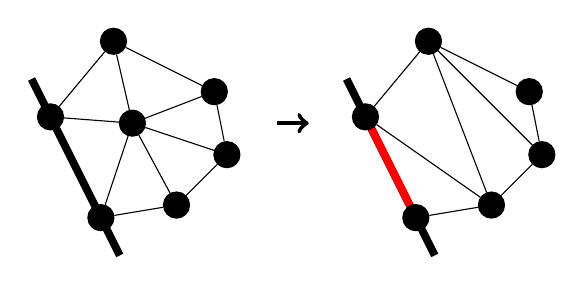
\begin{tikzpicture}[scale=.8,every node/.style={draw,shape=circle,fill=black,minimum size=3pt}]
% vertices
\path (0.5,1.5) node (p0) {}
(0,0) node (p1) {}
(1.2,0.2) node (p2) {}
(2,1) node (p3) {}
(1.8,2) node (p4) {}
(0.2,2.8) node (p5) {}
(-0.8,1.6) node (p6) {};
\path %(5.5,1.5) node (p7) {}
(5,0) node (p8) {}
(6.2,0.2) node (p9) {}
(7,1) node (p10) {}
(6.8,2) node (p11) {}
(5.2,2.8) node (p12) {}
(4.2,1.6) node (p13) {};
% edges
\draw (p0) -- (p1)
(p0) -- (p2)
(p0) -- (p3)
(p0) -- (p4)
(p0) -- (p5)
(p0) -- (p6)
(p1) -- (p2)
(p2) -- (p3)
(p3) -- (p4)
(p4) -- (p5)
(p5) -- (p6);
\draw [line width=0.1cm] (-1.1,2.2) -- (0.3,-0.6);
\draw (p8) -- (p9)
(p9) -- (p10)
(p10) -- (p11)
(p11) -- (p12)
(p12) -- (p13)
(p13) -- (p8)
(p9) -- (p13)
(p9) -- (p12)
(p10) -- (p12);
\draw [line width=0.1cm] (3.9,2.2) -- (5.3,-0.6);
\draw [line width=0.1cm,red] (p8) -- (p13);
% draw arrow
\draw [->,ultra thick] (2.8,1.5) -- (3.3,1.5);
\end{tikzpicture}
\label{fig:BoundaryReduction}
}
\caption{Reduction of polygons before and after eliminating the vertex. (a) General simple vertex case: number of polygons before reduction: $6$, number of polygons after reduction: $4$; (b) Boundary vertex case: number of polygons before reduction: $5$, number of polygons after reduction: $4$. Note that the edge in \emph{red} does not belong to the surface before the computation. }%
\label{fig:Reduction}
\end{figure}

To delete the unimportant vertices, some criteria must be designed and applied to validate the geometry of all potential targets among the model.
First of all, the complex vertices are definitely retained.
Then the rest are well checked to decide whether delete or not.
For the simple vertices that are not located on the boundary or the interior edge, the distance from them to the average plane is the unique principle -- if the distance is less than a certain value, it will be preserved; if not, it will be deleted. %
The vertices on the boundary or the interior edge are checked in the similar way -- if the distance is less than a certain value, it will be retained; otherwise, it will be kicked out. %
The vertices located at corners are usually preserved to maintain the approximation of the original geometry or left the ``noises" introduced in the modeling phase to be depressed by using appropriate method. %

Once upon the deletion of the vertex and its associated edges, one (in simple case) or two holes (in boundary or interior edge case) are left for patching thus maintaining the surface. In achieving the new patches for these holes, new triangulation at the location is created, which is done before the actual deletion mentioned before.

Comparing the number of triangles before and after this process, two triangles are reduced for the cases of general simple vertices, interior edge vertices, and some corner vertices; whilst one for the cases of vertices located at the boundaries (see Fig. \ref{fig:Reduction}). %

\section{Experiments and Results}

\subsection{Data and Experimental Setup}

The vasculature surface models were generated by applying the approaches proposed in \cite{Yang2014ICRA} from the original CTA images.
The resolution of the original data was $0.4 \times 0.4 \times 0.6 \text{mm}^3$.
For the sake of simplicity, only a segment of the abdominal aorta is depicted in this paper to demonstrate the effectiveness of our approach (see Fig. \ref{fig:VOI}).
The approach can be ported in order to process the model surfaces of the whole vasculature related to the surgical procedure to be simulated.

All of our experimental programs ran on a desktop machine equipped with Intel's 2.83GHz Core 2 Quad CPU and 4GB RAM.

\begin{figure}[t]
\centering
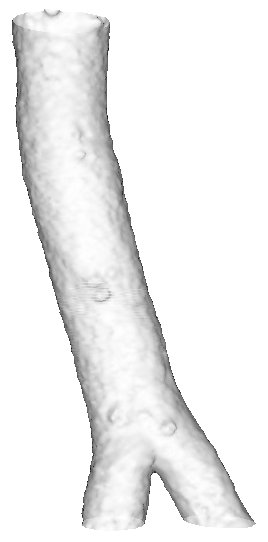
\includegraphics[height=2.0in]{Figures/chap06/original.png}
\caption{VOI-extracted surface model consisting of $74307$ polygons.}
\label{fig:VOI}
\end{figure}

\subsection{Validating Connectivity Between Vertices}

First of all, the polygonal elements in the patient-specific surface model of the human vessels need to be checked such that the connectivity between any pair of vertices are validated. %
After doing this, the integration of the model surface is guaranteed that the excessive polygons are kicked off.
Table \ref{tbl:Connectivity} shows that the total number of the polygonal surfaces were not changed, which implies that the given model (i.e., the local one) was already the largest-connected region in the model before the validation process. %

\subsection{Smoothing Model Surface}

Since the unavoidable noises introduced in the phase of image acquisition and processing, uneven surfaces may be found in the surface rendered based on the imagery.
The mess of artifacts and crusts may induce the problems in the smoothness of the delivery of the virtual surgical tools, e.g., guidewires, catheters, etc.
To avoid this situation, a thorough smoothing process is needed on the inner surface of the model, which is equivalent to the smoothing on the model surface per se.
\begin{table}[t]
\renewcommand{\arraystretch}{1.3}
\caption{Numbers of polygons before and after connectivity validation}
\label{tbl:Connectivity}
\centering
\begin{tabular}
{@{}l||r@{}}
%{@{}llrr@{}}
%\toprule
\hline
~                       & No. of polygons \\
\hline\hline
Before validation       & $74,307$  \\
After validation        & $74,307$  \\
\hline
\end{tabular}
\end{table}

The algorithm utilized in this processing task is implemented based on the low-pass filtering principles, with two parameters to be tuned in control of the smoothing effect on the objects. %
One of the parameters regulates the number of iterations the algorithm should take.
It is equivalent to the order of the polynomial that approximating the windowed sinc function given in (\ref{eqn:Approximation}).
The other parameter is used to configure the bandwidth of this so-called low-pass filter.

In this work, several parameter sets were given with the aim of searching for the one that can generate the most acceptable results.
The numbers of iterations of the smoothing were chosen to be $30$, $60$, and $100$ in the two cases, where the bandwidths were $0.1$, and $0.01$.

Judging from the resultant models in Fig. \ref{fig:Smooth}, the ones on the top row (see Figures \ref{fig:Smooth30-1}, \ref{fig:Smooth60-1}, and \ref{fig:Smooth100-1}) smoothed with the bandwidth $0.1$ are still fairly rough compared to the input, while the ones on the bottom row (see Figures \ref{fig:Smooth30-01}, \ref{fig:Smooth60-01}, and \ref{fig:Smooth100-01}) with the bandwidth $0.01$ are much better. %
With the increase of the number of iterations, the smoothing effect became more apparent, compared with the column of results from the one on its left.
At this stage of processing, we chose the parameter set which was used to generated the results depicted in Fig. \ref{fig:Smooth100-01} ($\text{no. of iterations} = 100$, $\text{pass band} = 0.01$). %
\begin{figure}[t]
\centering
\subfloat{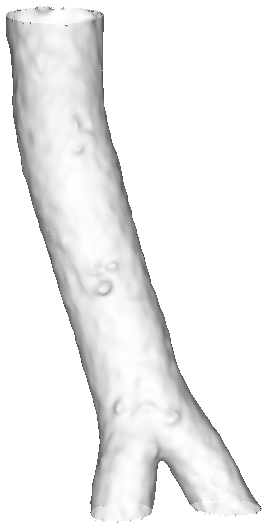
\includegraphics[height=2.0in]{Figures/chap06/smooth_30_1.png}%
\label{fig:Smooth30-1}}
\hfil
\subfloat{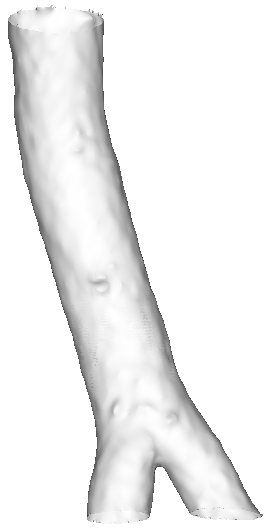
\includegraphics[height=2.0in]{Figures/chap06/smooth_60_1.png}%
\label{fig:Smooth60-1}}
\hfil
\subfloat{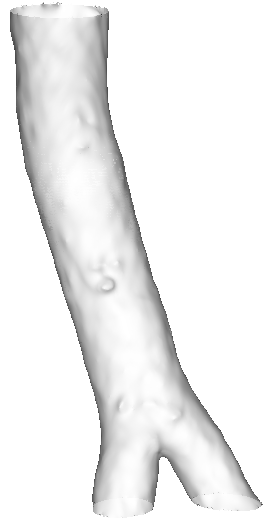
\includegraphics[height=2.0in]{Figures/chap06/smooth_100_1.png}%
\label{fig:Smooth100-1}}
\hfil
\subfloat{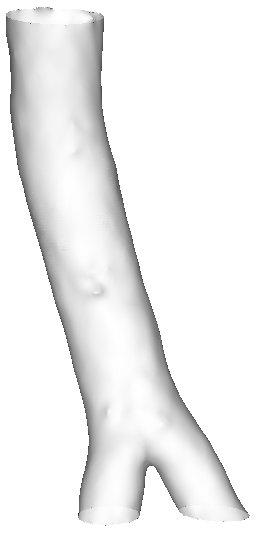
\includegraphics[height=2.0in]{Figures/chap06/smooth_30_01.png}%
\label{fig:Smooth30-01}}
\hfil
\subfloat{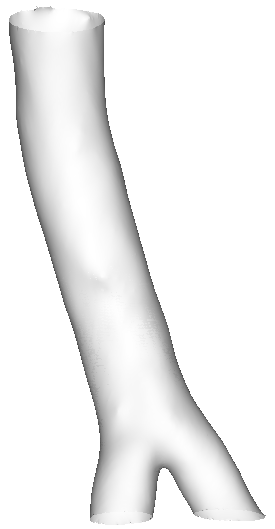
\includegraphics[height=2.0in]{Figures/chap06/smooth_60_01.png}%
\label{fig:Smooth60-01}}
\hfil
\subfloat{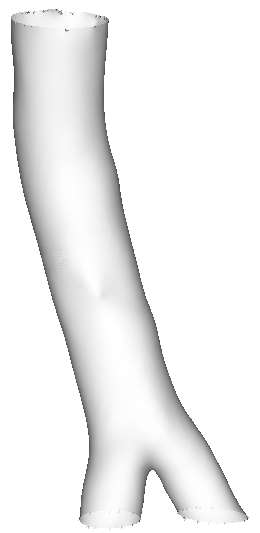
\includegraphics[height=2.0in]{Figures/chap06/smooth_100_01.png}%
\label{fig:Smooth100-01}}
\caption{Smoothing effects by applying different parameters: top row illustrate the results with $\text{pass band} = 0.1$, and the numbers of iterations are: $30$, $60$, and $100$, respectively; bottom row illustrate the results with $\text{pass band} = 0.01$, and the numbers of iterations are: $30$, $60$, and $100$, respectively.}%
\label{fig:Smooth}
\end{figure}

\subsection{Elimination of Component Polygons}

The elimination of polygon elements of the model surface was conducted after the smoothing computation terminated demonstrated in the last section.

For the input surface model, over $74$k polygons were required to model the vessel segment by using Marching Cubes method \cite{Lorensen1987MC}.
One can imagine that the overall number of the polygons needed to model the whole aorta and the trees of the coronary arteries.
Rendering the large amount of data will surely exhaust the most memory on any machine with typical hardware configuration, thus no sufficient space could be spared for the interaction and other computation.
To facilitate this situation, we adopted the decimation algorithm introduced in Section \ref{subsec:decimation} with multiple sets of parameters in a series of experiments. %

In this work, the termination conditions of the adopted algorithm were set to $10\%$, $50\%$, $75\%$, $90\%$, and $99\%$, respectively.
By termination condition, which is equivalent to the reduction rate, we mean that the rate of the total number of the polygonal elements deleted with respect to the total number of the polygonal elements in the input model surface. %
This can be written as follows
\begin{equation}
\label{eqn:ReductionRate}
\text{Reduction Rate (\%)} = \frac{\text{No. of \emph{deleted} Polygons}}{\text{No. of Input Polygons}}.
\end{equation}

Table \ref{tbl:Decimate} illustrates the effects of the decimation algorithm.
Figure \ref{fig:Decimate} depicts the visualization results of the decimation with typical parameters.
Observing the results, visualization in Figures \ref{fig:Decimate90} and \ref{fig:Decimate99} contain acceptable amounts of polygons.
However, the visualization in fig. \ref{fig:Decimate99} unveiled obvious alterations in its geometry.

\subsection{Discussions}

All the programs ran in the experiments were written in C++.
Some of the functioning modules were implemented based on the Visualization Toolkit (VTK) \cite{Schroeder2000VTK}, an open source effort containing various of computation facilities implementing algorithms from both the general and special fields of computer graphics. %

In validating the connectivity of the adjacent points among the surface model, the algorithm was configured to extract the largest-connected areas in this work.
To depress the effects from the noisy meshes introduced by image processing, a surface smoothing algorithm was employed to remove these meshes by slightly altering the locations of the vertices of the meshes. %
In smoothing the surface, two distinct parameters were the key switches for the algorithm, among which the width of the pass band of the low-pass filter and the number of the iterations to be performed were determined. %
Between the number of iterations and the smoothing effects on the surface, a positive correlation was demonstrated that the larger the number, the smoother the result.
On the other hand, the width of the pass band and the smoothing effects implied a negative correlation that the narrower the pass band, the smoother the result.
%One thing to be noted is that the loss of certain details occurred on all the resultant surface models.
\begin{table}[t]
\renewcommand{\arraystretch}{1.3}
\caption{Reduction rates and quantities of polygons in the model surface after decimation}
\label{tbl:Decimate}
\centering
\begin{tabular}{c||r r r r r}
\hline
%\bfseries      & \bfseries Quantity of polygonal surfaces \\
Reduction Rate ($\%$)  &    $10$ &    $50$ &    $75$ &   $90$ &  $99$ \\
\hline\hline
No. of Polygons & $66875$ & $37153$ & $18576$ & $7430$ & $743$ \\
\hline
\end{tabular}
\end{table}
\begin{figure}[t]
\centering
\subfloat{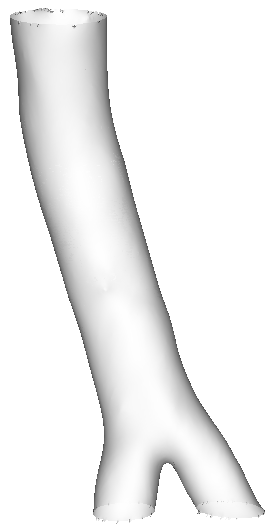
\includegraphics[height=2.0in]{Figures/chap06/smooth_100_01_d10.png}%
\label{fig:Decimate10}}
\hfil
\subfloat{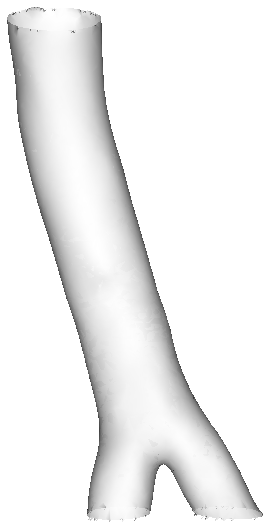
\includegraphics[height=2.0in]{Figures/chap06/smooth_100_01_d90.png}%
\label{fig:Decimate90}}
\hfil
\subfloat{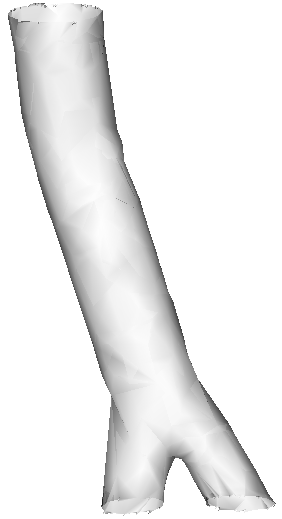
\includegraphics[height=2.0in]{Figures/chap06/smooth_100_01_d99.png}%
\label{fig:Decimate99}}
\hfil
\subfloat{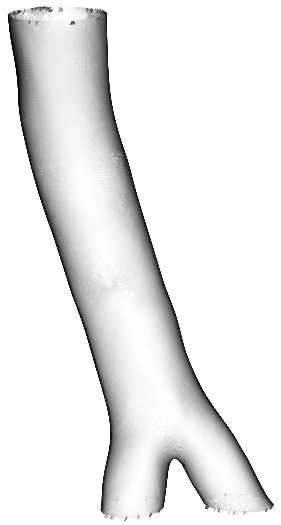
\includegraphics[height=2.0in]{Figures/chap06/smooth_100_01_d10_w.png}%
\label{fig:Decimate10-w}}
\hfil
\subfloat{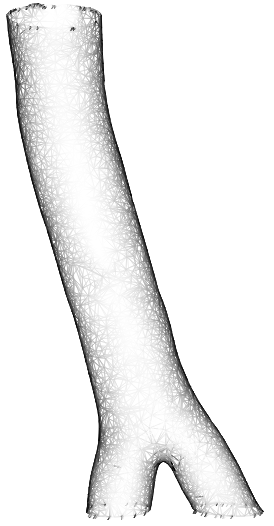
\includegraphics[height=2.0in]{Figures/chap06/smooth_100_01_d90_w.png}%
\label{fig:Decimate90-w}}
\hfil
\subfloat{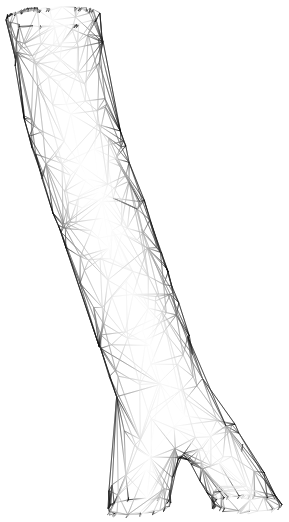
\includegraphics[height=2.0in]{Figures/chap06/smooth_100_01_d99_w.png}%
\label{fig:Decimate99-w}}
\caption{Decimation effects by applying different parameters: top row illustrate the results with reduction rates of $10\%$, $90\%$, and $99\%$, respectively; bottom row illustrate the wire frame representation of the corresponding results depicted above.}%
\label{fig:Decimate}
\end{figure}

In decimating the polygons, the problem is two-folded: on the one hand, the higher rate of reduction is preferred for the following interaction system; on the other hand, however, the over high rate of reduction may lead to heavy tortures on the model surface thus the geometry is doomed to be destroyed. %
This should be taken into consideration when selecting the reduction rate for the decimator algorithm.
In this work, we have tested series of cases with different rates and successfully determined the one that was acceptable in eliminating the excessive polygons.
The output of the decimation process are the progressive meshes \cite{Hoppe1996}.
Besides the aforementioned decimation on the input meshes, the resultant meshes had well preserved the geometry of the model, as well as its global appearance (normals, color values, etc.). %

\section{Conclusions and Future Work}
%The conclusion goes here.

In the context of simulating the intravascular surgical procedure, the interactive performance between the virtual surgical tools (i.e., catheters or guidewires) and the vasculature is one of the most important benchmarks. %
The amount of the data used to model the surface of the related vasculature is one of the main factors.
In this paper, we developed an approach in order to address this problem.
The basic idea is to eliminate the polygon components consisting the model surface without destroying the geometry of the vasculature.
The data used in the experiments were the patient-specific vessel model generated by series of image processing on the original CT dataset in our previous work.

First of all, the connectivity between the adjacent vertices was validated and the unconnected vertices were removed.
Then the noisy surfaces introduced from the image acquisition and processing were smoothed with the least effects on the model's geometry.
Finally the decimation pass was introduced to reduce the number of the polygon components at the desired reduction rate.
In reducing the polygonal elements, not only did we consider the number of the polygons that had been removed, but also the visualization of the resultant models.
Experimental results illustrated the effectiveness of our approach in reducing the quantities of the polygonal elements in the surface model.

Our future work will be the visualization of other human organs (e.g., heart, skeletons, etc.) appeared in the field of real surgeries on the one hand, and the physical modeling of the virtual human organs on the other. %
